\section{Murmuration of Elliptic Curves}
\label{sec:elliptic}

\subsection{He--Lee--Oliver--Pozdnyakov's Murmuration}
\label{subsec:elliptic_hlop}

Murmuration of elliptic curves refers to the following average of Frobenius traces.
Fix a nonnegative integer $r$ and $N_1 < N_2$.
Let $\cE_r[N_1, N_2]$ be the set of isomorphism classes of elliptic curves $E_{/\bQ}$ with conductor $N(E) \in [N_1, N_2]$ and rank $r$.
For a fixed prime $p$, we consider the following average
\begin{equation}
    \bE_{E \in \cE_r[N_1, N_2]} [a_p(E)] = \frac{\sum_{E \in \cE_r[N_1, N_2]} a_p(E)}{\sum_{E \in \cE_r[N_1, N_2]} 1}
\end{equation}
as a function of $p$.
What He, Lee, Oliver, and Pozdnyakov \cite{he2024murmurations} observed is that this yields a surprising oscillation pattern as in Figure \ref{fig:hlop}.
Especially, it appears to have the same oscillation pattern for different conductor ranges, where the pattern seems to only depend on the rank $r$.

\begin{figure}[htp] 
\centering
    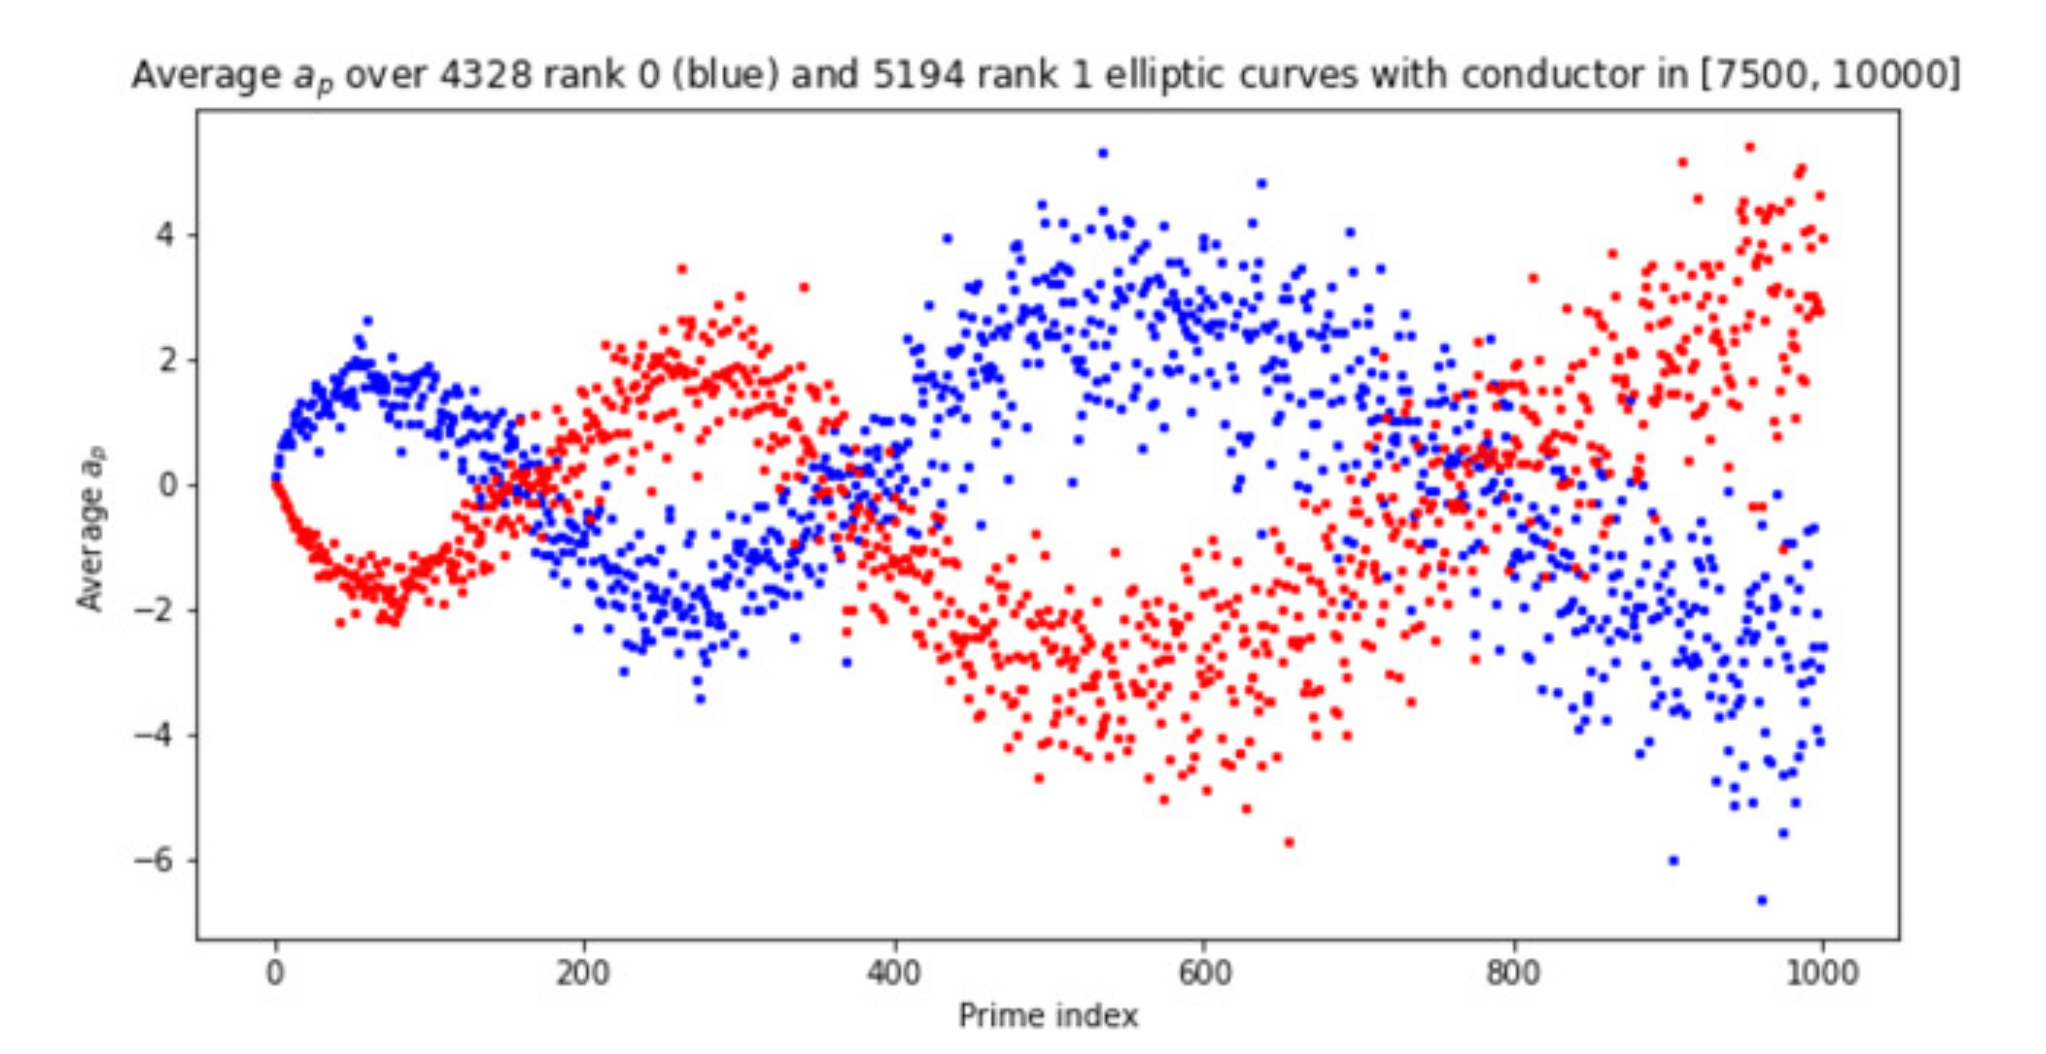
\includegraphics[width=0.7\textwidth]{src/hlop.png}%
    \caption{Murmuration of elliptic curves with conductor in $[7500, 1000]$ and rank $r = 0$ (blue) and $r = 1$ (red) \cite{he2024murmurations}.}
\label{fig:hlop}
\end{figure}


\subsection{Sutherland's observation}
\label{subsec:elliptic_sutherland}

Later, Sutherland \cite{sutherlandletter} (and further works by several people) showed that one really needs to view the murmuration density as a function of $p / N$ rather than $p$ for a fixed $N$.
He found that, for different dyadic intervals of the form $(2^k, 2^{k+1}]$, the murmuration patterns look the same (and become clearer as $k$ increases), even if the averages consider completely different sets of elliptic curves (Figure \ref{fig:sutherland_elliptic_dyadic}).
Also, instead of considering each rank separately, it seems better to consider all ranks together, where we weight $a_p(E)$ by the root number $\epsilon(E)$ of $E$.
One can separate into two groups depending on the parity of the rank.
So the major open question is to \emph{compute} the density function, i.e. to find a function $M: (0, \infty) \to \bR$ such that
\begin{equation}
    \bE_{E \in \cE_r[N, 2N]} [a_p(E)] = M\left(\frac{p}{N}\right) + \text{error}
\end{equation}
where the error term goes to zero as $N \to \infty$. More generally, one can fix $0 < C_1 < C_2$ and consider the interval $[C_1 N, C_2 N]$.

\begin{figure}[htp] 
    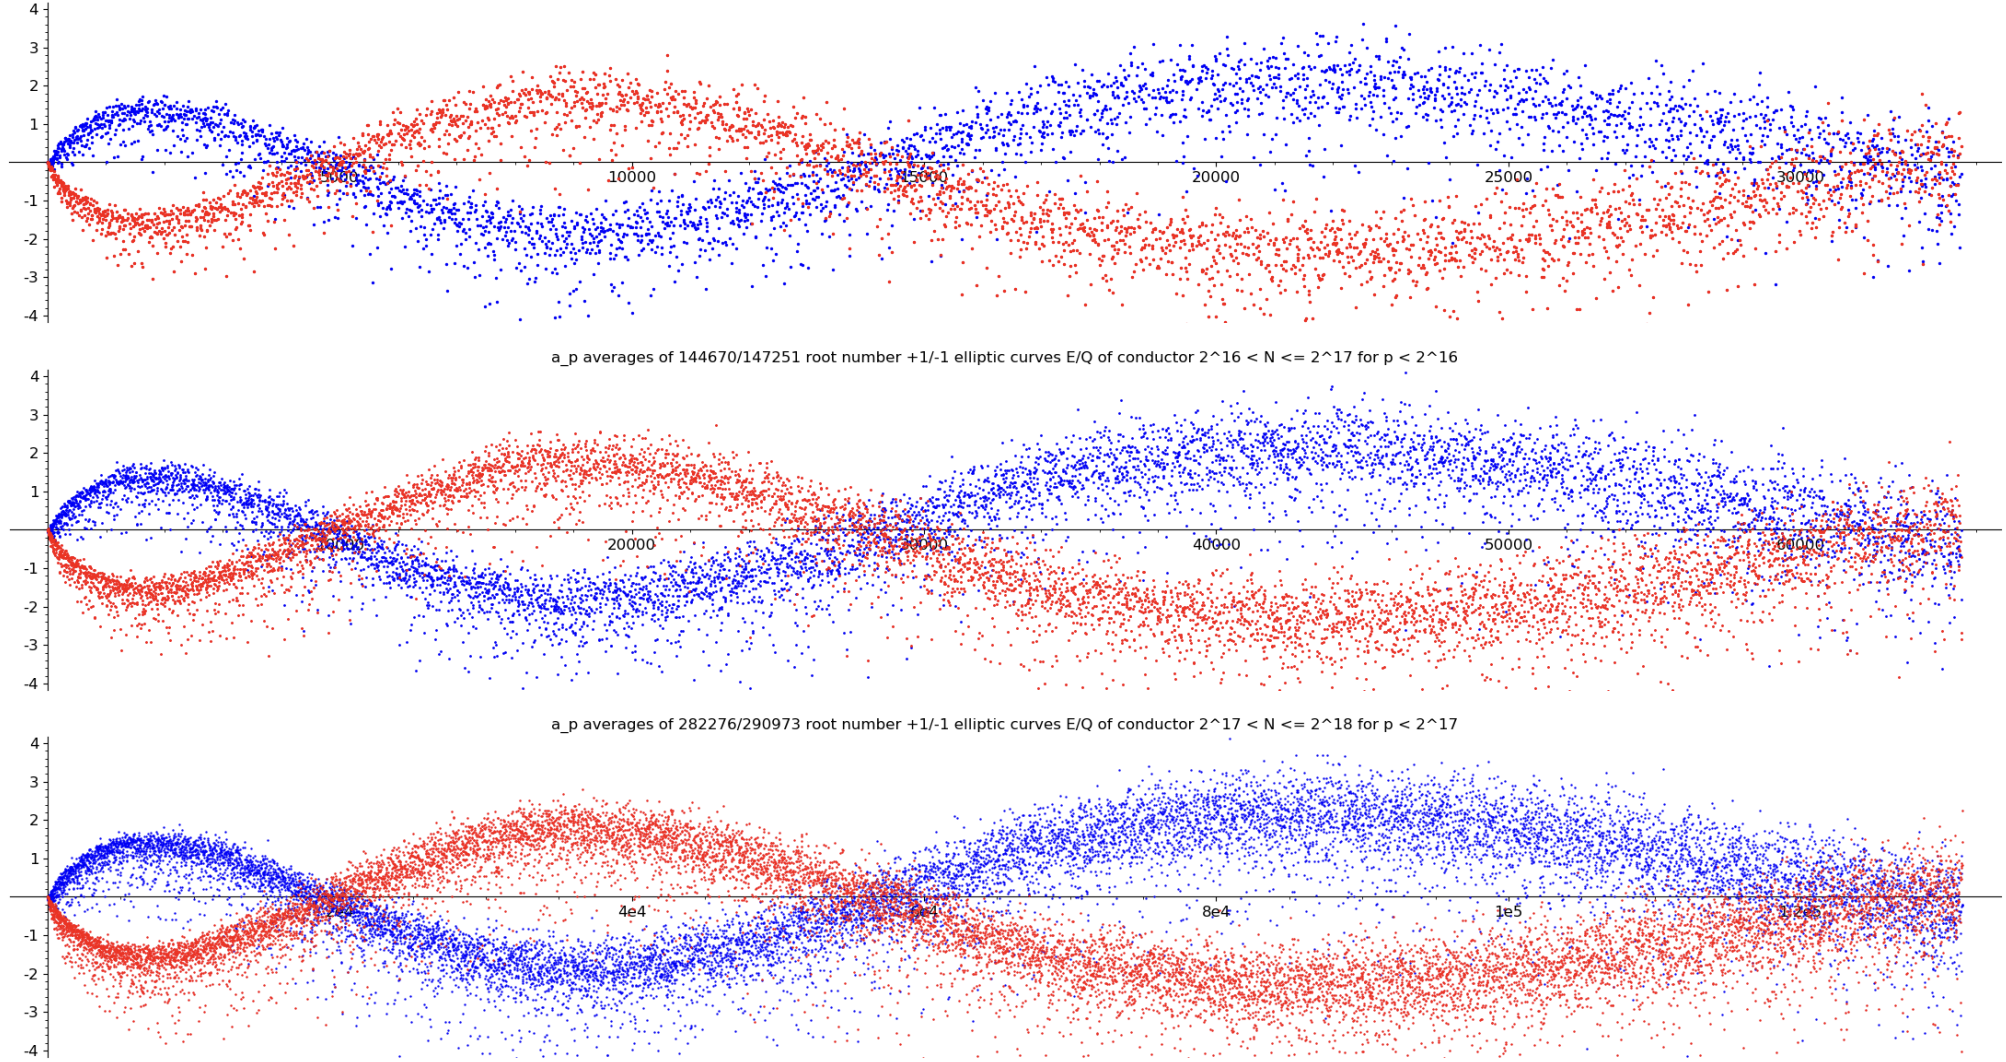
\includegraphics[width=\textwidth]{src/sutherland.png}%
    \caption{Murmuration of elliptic curves with conductor in $[2^{k}, 2^{k+1})$ and primes $p < 2^{k-1}$ for $k = 15, 16, 17$ \cite{sutherlandletter}. Blue (resp. red) curves correspond to $\epsilon(E) = +1$ (resp. $-1$) elliptic curves.}
\label{fig:sutherland_elliptic_dyadic}
\end{figure}


Sutherland also observed that the murmuration disappears when elliptic curves are ordered by other measures, such as naive height, discriminant, or $j$-invariants, although further local averaging gives murmuration for naive heights (see Section \ref{sec:elliptic2}).
This shows that the murmuration is a phenomenon that is sensitive to the ordering of elliptic curves.


\subsection{What is the role of Machine Learning?}

Although there seems to be no machine learning involved in the previous discussions, I will make a brief comment on the relation between machine learning and murmuration, as I found that existing literature is often misleading in distinguishing the machine learning part from the murmuration part.
I have read a few articles on the internet which basically say that ``AI found new mathematics,'' which is false.

One of the main motivations of the paper \cite{he2024murmurations} is to study elliptic curves via machine learning.
Especially, they were interested in predicting the rank of elliptic curves (which is widely known to be hard to compute in general) by means of machine learning, where the coefficients $a_p(E)$ of Hasse--Weil $L$-functions are used as features.
Surprisingly, they found that a simple logistic regression model can already distinguish between rank $0$ and $1$ elliptic curves with high accuracy of $>90\%$ (see also \cite{he2023machine}).
Along these lines, they (more precisely, He, Lee, and Oliver) were curious about what was actually going on, and Pozdnyakov (who was an undergraduate student of Lee at that time) figured out the murmuration pattern.
This somehow gives an explanation for the high accuracy of the model, since the murmuration patterns for rank $0$ and $1$ elliptic curves are noticeably different.
But the correct way to say it is that the machine learning experiments \emph{motivated} them to study what the models were doing, which is essentially the work of humans, not the ML models.
You can find more of the story in the Quanta Magazine article \cite{chiou2024elliptic}.

% and they conjectured that the murmuration density is related to the rank of elliptic curves.

\subsection{Sato--Tate conjecture and Murmuration}


One should not confuse murmuration with the (vertical) Sato--Tate conjecture, which we will explain here.
The original (i.e. \emph{horizontal}) Sato--Tate conjecture is about the distribution of $a_p(E)$ for a \emph{fixed $E_{/\bQ}$ and varying $p$}.
The Hasse--Weil bound says that $|a_p(E)| \le 2 \sqrt{p}$, and the conjecture predicts that for a non-CM elliptic curve $E$, the distribution of $a_p(E)$ is semicircular with radius $2\sqrt{p}$, i.e., the density function is $\frac{1}{2\pi}\sqrt{4 - x^2} \dd x$ for the normalized traces $a_p(E)/\sqrt{p}$.
Equivalently, if we write $a_p(E) = 2 \sqrt{p} \cos \theta_p$ for $\theta_p \in [0, \pi]$, then $\theta_p$ follows the distribution $\frac{2}{\pi} \sin^2 \theta \dd \theta$.
The distributions for CM elliptic curves are different, and we also expect that the Frobenius traces for abelian varieties of higher dimension will follow certain distributions, which are conjecturally the pushforward of the Haar measure of a certain compact Lie group, called the \emph{Sato--Tate group}.
See \cite{sutherland2019sato} for more about the Sato--Tate conjecture and recent progress on it.


The \emph{vertical} Sato--Tate conjecture fixes $p$ and varies $E$ over $\bF_p$ instead, where there are only finitely many isomorphism classes of $E$ over $\bF_p$.
Birch \cite{birch1968number} proved that the distribution converges to the above semicircular distribution as $p \to \infty$.
This is different from the murmuration for two reasons: vertical Sato--Tate considers the elliptic curves over $\bF_p$, and there's no conductor involved in vertical Sato--Tate.
